\documentclass[12pt]{article}
\usepackage{a4wide, amsfonts, epsfig,bbding}

\begin{document}
\begin{center}
{\bf EMAT10001 Lecture 13.}\\[1cm]{} Conor Houghton 2014-1-25
\end{center}
\subsection*{Preface} 
These are outline notes for lecture 5. As usual there is a bounty of
between 20p and \pounds 2 for errors, you can tell me at the end of a
lecture or email me at \texttt{conor.houghton{@}bristol.ac.uk}.

\subsection*{Introduction}

This lecture is about the exponential and about simple differential
equations, well mostly one differential equation, the growth equation,
which models the dynamics of growth and decay.

\subsection*{The limit of continuous compounding}
Imagine you have money in a bank, say 1000 euro at 10\% interest per
annum; this example is set quite a few years ago. After one year you
get your interest and you'll have 1100 euro. However, this isn't quite
fair, what would happen if the bank gave you your interest every six
months; 5\% per semiannum. In this system after six months you would
get 50 euro giving you 1050 euro, and after another six months you
would get 5\% of this, giving you 1102.50 euro, an extra 2.50
euro. How about doing the interest every three months; then you would
have 1025 euro after three months, 1050.625 euro after six months,
about 1076.90 after nine months and 1103.82 after the full year, an
extra 3.82 euro.

Now lets think about the limit, where you continually add the
interest. If the interest rate is $r$, written as a fraction, and $P$
is the amount of money you are adding interest to, then the interest
is $rP$ and so after the interest is added you have $P+rP=(1+r)P$; in
other words, adding the interest is like multiplying by $(1+r)$. Writing the amount after interest is added as $P_1$, one since it added only once at the end of the year, we have
\begin{equation}
P_1=(1+r)P
\end{equation}
If it is added every six months, the interest is $r/2$ and
\begin{equation}
P_2=\left(1+\frac{r}{2}\right)\left(1+\frac{r}{2}\right)P=\left(1+\frac{r}{2}\right)^2P
\end{equation}
Now, by the same argument adding the interest $n$ times gives 
\begin{equation}
P_n=\left(1+\frac{r}{n}\right)^nP
\end{equation}

It turns out you can take the limit as $n$ goes to infinity, often
called the \textsl{limit of continual compounding}. The name given to
this limit is the exponential function:
\begin{equation}
\exp{r}=\lim{n\rightarrow \infty}\left(1+\frac{r}{n}\right)^n
\end{equation}
and so after one year you should get
\begin{equation}
P_\infty=\exp{r}P
\end{equation}
or, for our case, 1105.17 euro.

Now, what about the properties of this exponential function? First
off, lets differenciate it
\begin{equation}
\frac{d}{dx}\exp{(x)}=\lim_{n\rightarrow \infty}\frac{d}{dx}\left(1+\frac{x}{n}\right)^n=\lim_{n\rightarrow \infty}\frac{x}{n}n\left(1+\frac{x}{n}\right)^{n-1}
\end{equation}
where we have used the chain rule
\begin{equation}
\frac{d}{dx}f(g(x))=\frac{d}{dx}g(x)\frac{d}{dg}f(g)
\end{equation}
In this case that means we want $df/dx$ where 
\begin{equation}
f(x)=\left(1+\frac{x}{n}\right)^n
\end{equation}
or
\begin{equation}
f(x)=g(x)^n
\end{equation}
where
\begin{equation}
g(x)=\left(1+\frac{x}{n}\right)
\end{equation}
so 
\begin{equation}
\frac{df}{dg}=ng^{n-1}
\end{equation}
and
\begin{equation}
\frac{dg}{dx}=\frac{1}{n}
\end{equation}
Now, going back to where we started, 
\begin{equation}
\frac{d}{dx}\exp{(x)}=\lim_{n\rightarrow \infty}\frac{1}{n}n\left(1+\frac{x}{n}\right)^{n-1}
\end{equation}
and, since there is no difference between $n$ and $n-1$ when $n$ is going to infinity, we have
\begin{equation}
\frac{d}{dx}\exp(x)=\exp(x)
\end{equation}
This is the signature property of the exponential, differentiating it
gives you back the same function.

We can use this to work out how to calculate the exponential function. Say 
\begin{equation}
\exp(x)=\sum_{i=0}^\infty a_ix^i
\end{equation}
for some constants $a_i$, now
\begin{equation}
\frac{d}{dx}\exp(x)=\frac{d}{dx}\sum_{i=0}^\infty a_ix^i=\sum_{i=0}^\infty ia_ix^{i-1}
\end{equation}
so the equation $d\exp(x)/dx=\exp(x)$ tells us that
\begin{equation}
\sum_{i=0}^\infty a_ix^i=\sum_{i=0}^\infty ia_ix^{i-1}
\end{equation}
We want to solve this for the $a_i$, to do this we have to change the index in the second sum, so we write $j=i-1$ and put it back in
\begin{equation}
\sum_{i=0}^\infty a_ix^i=\sum_{j=-1}^\infty (j+1)a_{j+1}x^{j}
\end{equation}
then, just like it doesn't matter what you call a local variable in a for loop, it doesn't matter what you call an index in a sum, so we can write
\begin{equation}
\sum_{i=0}^\infty a_ix^i=\sum_{i=-1}^\infty (i+1)a_{i+1}x^{i}
\end{equation}
Now, when $i=-1$ we have $i+1=0$ so the $i=-1$ term in the right hand side sum can be ignored, giving
\begin{equation}
\sum_{i=0}^\infty a_ix^i=\sum_{i=0}^\infty (i+1)a_(i+1)x^{i}
\end{equation}
and, finally,
\begin{equation}
\sum_{i=0}^\infty [a_i-(i+1)a_{i+1}]x^i=\sum_{i=0}^\infty (i+1)a_{i+1}x^{i}
\end{equation}
so 
\begin{equation}
a_{i+1}=\frac{1}{i+1}a_i
\end{equation}
Finally, from
\begin{equation}
\exp(x)=\lim{n\rightarrow \infty}\left(1+\frac{x}{n}\right)^n
\end{equation}
we can see $\exp(0)=1$ and hence $a_0=1$, then from the formula
\begin{equation}
a_1=a_0
\end{equation}
and 
\begin{equation}
a_2=\frac{1}{2}a_1=\frac{1}{2}
\end{equation}
and
\begin{equation}
a_3=\frac{1}{3}a_2=\frac{1}{3!}
\end{equation}
and so on. Hence
\begin{equation}
\exp(x)=1+x+\frac{1}{2}x^2+\frac{1}{3!}x^3+\frac{1}{4!}x^4+\frac{1}{5!}x^5+\ldots
\end{equation}

One thing that isn't obvious from all of this, but which can be proven by messing around with the power series above, the exponential has the form of a power
\begin{equation}
\exp(x)=e^{x}
\end{equation}
where $e$ is a special number
\begin{equation}
e=\lim_{n\rightarrow \infty}\left(1+\frac{1}{n}\right)^n= 2.7182818283\ldots
\end{equation}
Like $\pi$ this is not a rational number, it isn't of the form $n/m$
for any $n$ and $m$; and, again like $\pi$, it is
\textsl{transendental}; it isn't the solution of any polynomial
equation with rational coefficients.

Now, consider the following common type of situation; you have a
quantity of bacteria, say 0.25 kg and each cell has $0.1$ chance of
dividing into two every hour; the challenge is to work out the
quantity of bacteria after a 24 hours. Now, call the quantity of
bacteria $P$ and the rate of change of the quantity is
\begin{equation}
\frac{dP}{dt}=rP
\end{equation}
where $r=0.1$ and we are measuring $t$ in hours; notice that it is
$rP$, the rate of change is the probability of a given bacteria
dividing multiplied by the total quantity of bacteria. To do this we
need to solve the equation. There are lots of ways to solve
differential equations like this but, perhaps, the best way is to
guess based on our knowledge of exponentials; broadly speaking this is
called the method of ansatze. Hence, we guess the solution might be
\begin{equation}
P(t)=Ae^{st}
\end{equation}
where $A$ and $s$ are constants. Now
\begin{equation}
\frac{d}{dt}P(t)=A\frac{d}{dt}e^{st}
\end{equation}
and using the chain rule again, that give 
\begin{equation}
\frac{d}{dt}P(t)=Ase^{st}
\end{equation}
so substituting into the differential equation we have
\begin{equation}
Ase^{st}=rAe^{st}
\end{equation}
so that's a solution provided $s=r$. We also have to consider the initial condition $P(0)=0.25$, substituting $t=0$ into our solution we have
\begin{equation}
P(0)=A=0.25
\end{equation}
and
\begin{equation}
P(t)=0.25e^{0.1t}
\end{equation}
so $P(24)=0.25\exp(2.4)\approx 2.756$ and the growth is plotted in Fig.~1.
\begin{figure}
\begin{center}
% GNUPLOT: LaTeX picture with Postscript
\begingroup
  \makeatletter
  \providecommand\color[2][]{%
    \GenericError{(gnuplot) \space\space\space\@spaces}{%
      Package color not loaded in conjunction with
      terminal option `colourtext'%
    }{See the gnuplot documentation for explanation.%
    }{Either use 'blacktext' in gnuplot or load the package
      color.sty in LaTeX.}%
    \renewcommand\color[2][]{}%
  }%
  \providecommand\includegraphics[2][]{%
    \GenericError{(gnuplot) \space\space\space\@spaces}{%
      Package graphicx or graphics not loaded%
    }{See the gnuplot documentation for explanation.%
    }{The gnuplot epslatex terminal needs graphicx.sty or graphics.sty.}%
    \renewcommand\includegraphics[2][]{}%
  }%
  \providecommand\rotatebox[2]{#2}%
  \@ifundefined{ifGPcolor}{%
    \newif\ifGPcolor
    \GPcolorfalse
  }{}%
  \@ifundefined{ifGPblacktext}{%
    \newif\ifGPblacktext
    \GPblacktexttrue
  }{}%
  % define a \g@addto@macro without @ in the name:
  \let\gplgaddtomacro\g@addto@macro
  % define empty templates for all commands taking text:
  \gdef\gplbacktext{}%
  \gdef\gplfronttext{}%
  \makeatother
  \ifGPblacktext
    % no textcolor at all
    \def\colorrgb#1{}%
    \def\colorgray#1{}%
  \else
    % gray or color?
    \ifGPcolor
      \def\colorrgb#1{\color[rgb]{#1}}%
      \def\colorgray#1{\color[gray]{#1}}%
      \expandafter\def\csname LTw\endcsname{\color{white}}%
      \expandafter\def\csname LTb\endcsname{\color{black}}%
      \expandafter\def\csname LTa\endcsname{\color{black}}%
      \expandafter\def\csname LT0\endcsname{\color[rgb]{1,0,0}}%
      \expandafter\def\csname LT1\endcsname{\color[rgb]{0,1,0}}%
      \expandafter\def\csname LT2\endcsname{\color[rgb]{0,0,1}}%
      \expandafter\def\csname LT3\endcsname{\color[rgb]{1,0,1}}%
      \expandafter\def\csname LT4\endcsname{\color[rgb]{0,1,1}}%
      \expandafter\def\csname LT5\endcsname{\color[rgb]{1,1,0}}%
      \expandafter\def\csname LT6\endcsname{\color[rgb]{0,0,0}}%
      \expandafter\def\csname LT7\endcsname{\color[rgb]{1,0.3,0}}%
      \expandafter\def\csname LT8\endcsname{\color[rgb]{0.5,0.5,0.5}}%
    \else
      % gray
      \def\colorrgb#1{\color{black}}%
      \def\colorgray#1{\color[gray]{#1}}%
      \expandafter\def\csname LTw\endcsname{\color{white}}%
      \expandafter\def\csname LTb\endcsname{\color{black}}%
      \expandafter\def\csname LTa\endcsname{\color{black}}%
      \expandafter\def\csname LT0\endcsname{\color{black}}%
      \expandafter\def\csname LT1\endcsname{\color{black}}%
      \expandafter\def\csname LT2\endcsname{\color{black}}%
      \expandafter\def\csname LT3\endcsname{\color{black}}%
      \expandafter\def\csname LT4\endcsname{\color{black}}%
      \expandafter\def\csname LT5\endcsname{\color{black}}%
      \expandafter\def\csname LT6\endcsname{\color{black}}%
      \expandafter\def\csname LT7\endcsname{\color{black}}%
      \expandafter\def\csname LT8\endcsname{\color{black}}%
    \fi
  \fi
  \setlength{\unitlength}{0.0500bp}%
  \begin{picture}(5040.00,3528.00)%
    \gplgaddtomacro\gplbacktext{%
      \csname LTb\endcsname%
      \put(682,1207){\makebox(0,0)[r]{\strut{} 2}}%
      \put(682,1782){\makebox(0,0)[r]{\strut{} 4}}%
      \put(682,2357){\makebox(0,0)[r]{\strut{} 6}}%
      \put(682,2932){\makebox(0,0)[r]{\strut{} 8}}%
      \put(814,484){\makebox(0,0){\strut{} 0}}%
      \put(1346,484){\makebox(0,0){\strut{} 5}}%
      \put(1878,484){\makebox(0,0){\strut{} 10}}%
      \put(2409,484){\makebox(0,0){\strut{} 15}}%
      \put(2941,484){\makebox(0,0){\strut{} 20}}%
      \put(3473,484){\makebox(0,0){\strut{} 25}}%
      \put(4005,484){\makebox(0,0){\strut{} 30}}%
      \put(4537,484){\makebox(0,0){\strut{} 35}}%
      \put(176,1983){\rotatebox{-270}{\makebox(0,0){\strut{}$P$ (kg)}}}%
      \put(2728,154){\makebox(0,0){\strut{}$t$ (hours)}}%
    }%
    \gplgaddtomacro\gplfronttext{%
    }%
    \gplbacktext
    \put(0,0){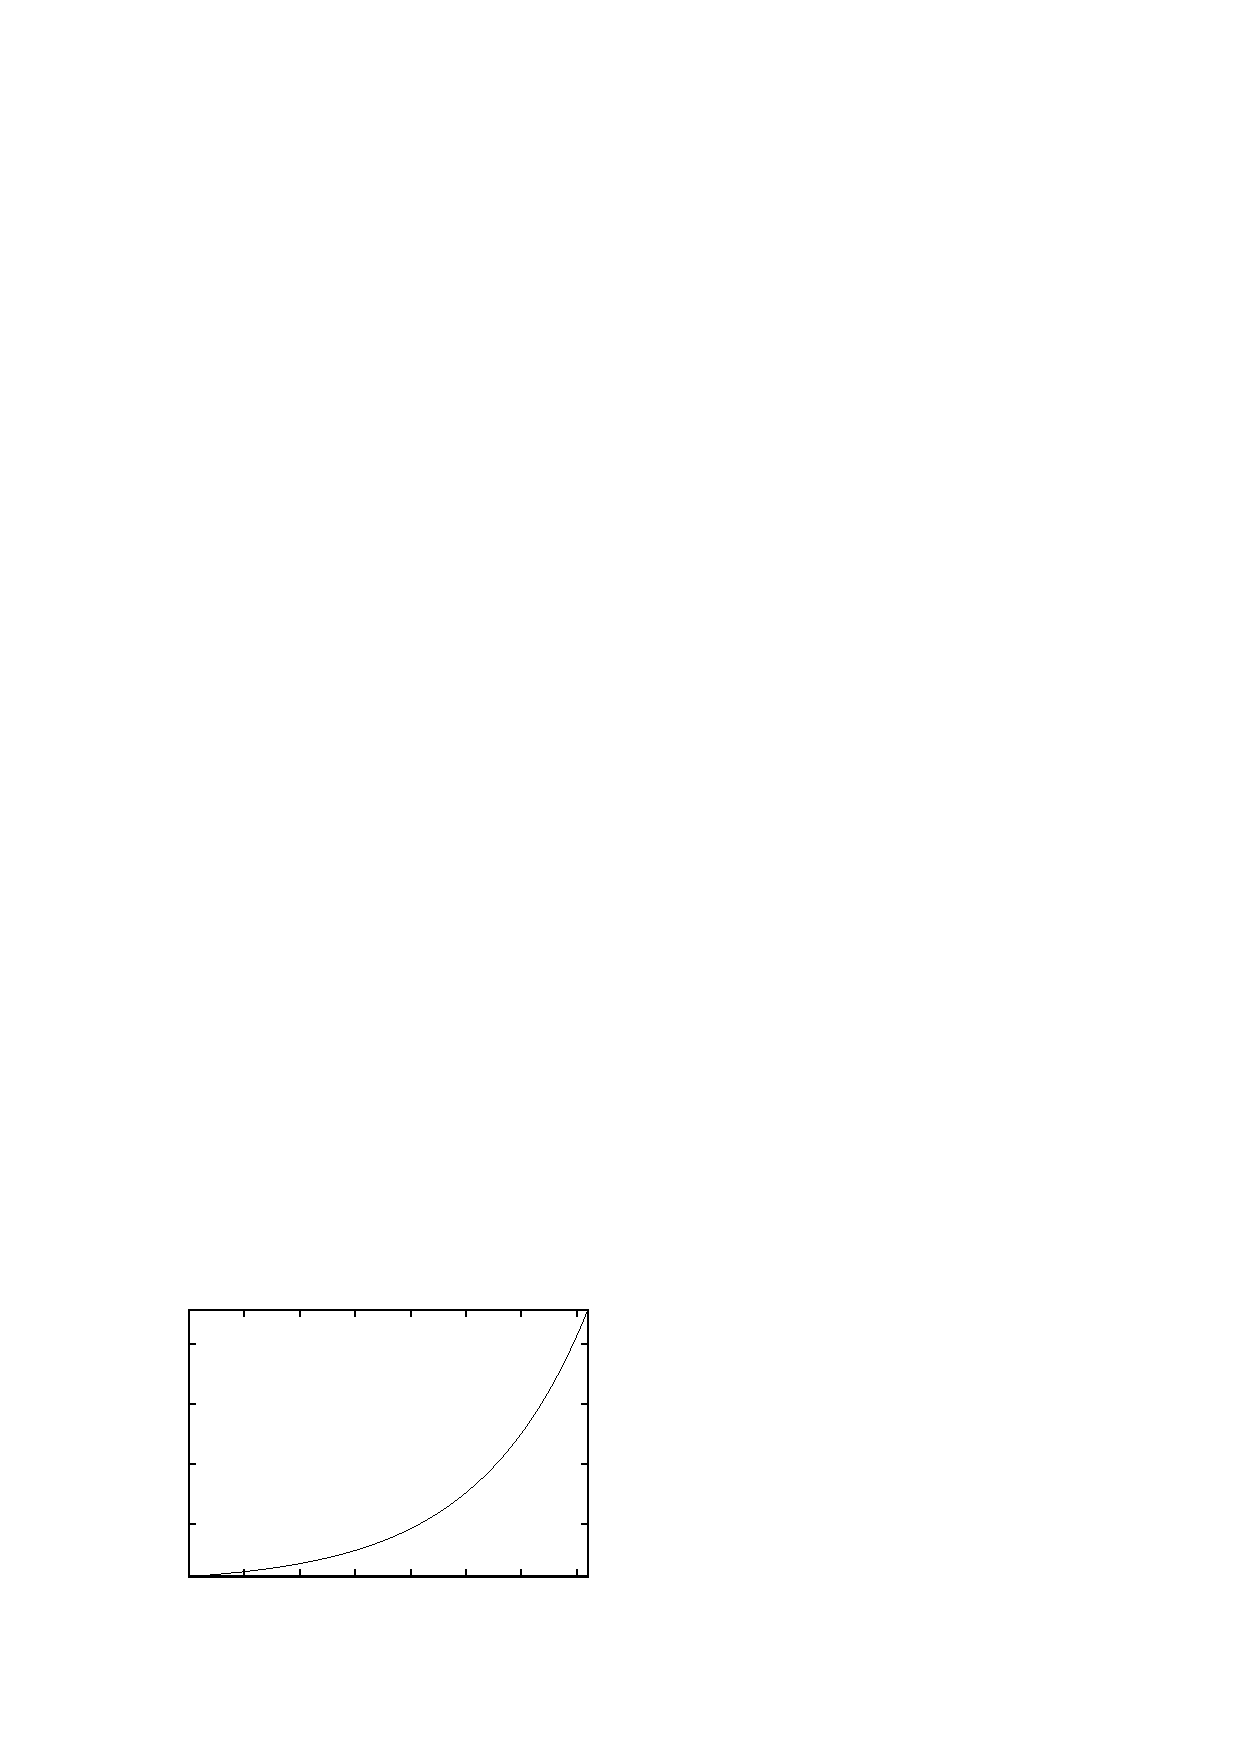
\includegraphics{lecture13_exp}}%
    \gplfronttext
  \end{picture}%
\endgroup

\end{center}
\caption{Plot of $0.25\exp(0.1t)$.}
\end{figure}


\end{document}


